\documentclass[tikz]{standalone}

\begin{document}

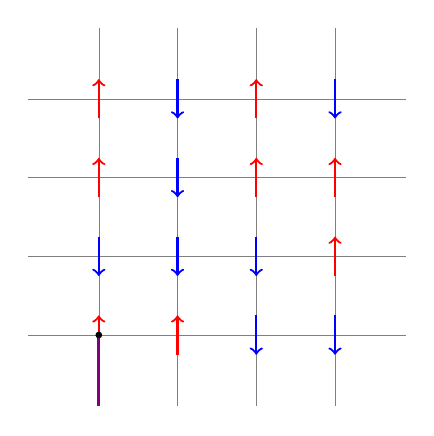
\begin{tikzpicture}
    % grid
    \draw[step=1cm, gray, very thin] (0.1, 0.1) grid (4.9, 4.9);
    % row 1
    \draw[red, ->, thick] (1, 0.75) -- (1, 1.25);
    \draw[red, ->, thick] (2, 0.75) -- (2, 1.25);
    \draw[blue, ->, thick] (3, 1.25) -- (3, 0.75);
    \draw[blue, ->, thick] (4, 1.25) -- (4, 0.75);
    % row 2    
    \draw[blue, ->, thick] (1, 2.25) -- (1, 1.75);
    \draw[blue, ->, thick] (2, 2.25) -- (2, 1.75);
    \draw[blue, ->, thick] (3, 2.25) -- (3, 1.75);
    \draw[red, ->, thick] (4, 1.75) -- (4, 2.25);
    % row 3
    \draw[red, ->, thick] (1, 2.75) -- (1, 3.25);
    \draw[blue, ->, thick] (2, 3.25) -- (2, 2.75);
    \draw[red, ->, thick] (3, 2.75) -- (3, 3.25);
    \draw[red, ->, thick] (4, 2.75) -- (4, 3.25);
    % row 4
    \draw[red, ->, thick] (1, 3.75) -- (1, 4.25);
    \draw[blue, ->, thick] (2, 4.25) -- (2, 3.75);
    \draw[red, ->, thick] (3, 3.75) -- (3, 4.25);
    \draw[blue, ->, thick] (4, 4.25) -- (4, 3.75);
    % worm
    \draw[violet, very thick] (1, 0.1) -- (1, 1);
    \filldraw (1, 1) circle (1pt);
\end{tikzpicture}

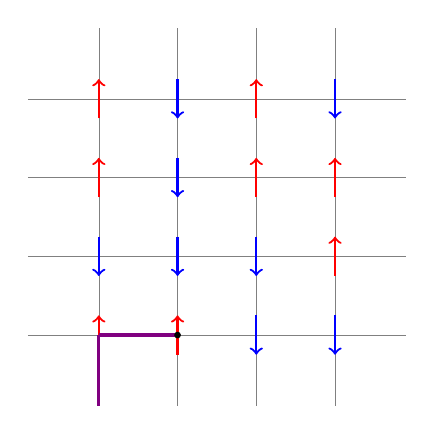
\begin{tikzpicture}
    % grid
    \draw[step=1cm, gray, very thin] (0.1, 0.1) grid (4.9, 4.9);
    % row 1
    \draw[red, ->, thick] (1, 0.75) -- (1, 1.25);
    \draw[red, ->, thick] (2, 0.75) -- (2, 1.25);
    \draw[blue, ->, thick] (3, 1.25) -- (3, 0.75);
    \draw[blue, ->, thick] (4, 1.25) -- (4, 0.75);
    % row 2    
    \draw[blue, ->, thick] (1, 2.25) -- (1, 1.75);
    \draw[blue, ->, thick] (2, 2.25) -- (2, 1.75);
    \draw[blue, ->, thick] (3, 2.25) -- (3, 1.75);
    \draw[red, ->, thick] (4, 1.75) -- (4, 2.25);
    % row 3
    \draw[red, ->, thick] (1, 2.75) -- (1, 3.25);
    \draw[blue, ->, thick] (2, 3.25) -- (2, 2.75);
    \draw[red, ->, thick] (3, 2.75) -- (3, 3.25);
    \draw[red, ->, thick] (4, 2.75) -- (4, 3.25);
    % row 4
    \draw[red, ->, thick] (1, 3.75) -- (1, 4.25);
    \draw[blue, ->, thick] (2, 4.25) -- (2, 3.75);
    \draw[red, ->, thick] (3, 3.75) -- (3, 4.25);
    \draw[blue, ->, thick] (4, 4.25) -- (4, 3.75);
    % worm
    \draw[violet, very thick] (1, 0.1) -- (1, 1);
    \draw[violet, very thick] (1, 1) -- (2, 1);
    \filldraw (2, 1) circle (1pt);
\end{tikzpicture}

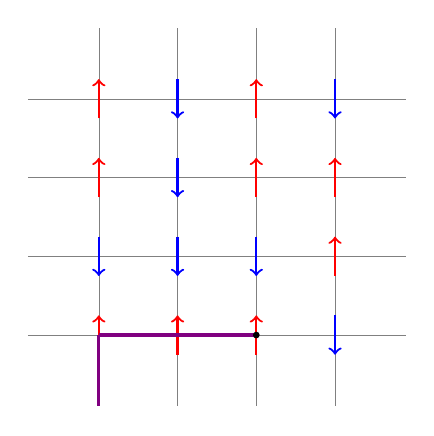
\begin{tikzpicture}
    % grid
    \draw[step=1cm, gray, very thin] (0.1, 0.1) grid (4.9, 4.9);
    % row 1
    \draw[red, ->, thick] (1, 0.75) -- (1, 1.25);
    \draw[red, ->, thick] (2, 0.75) -- (2, 1.25);
    \draw[red, ->, thick] (3, 0.75) -- (3, 1.25);
    \draw[blue, ->, thick] (4, 1.25) -- (4, 0.75);
    % row 2    
    \draw[blue, ->, thick] (1, 2.25) -- (1, 1.75);
    \draw[blue, ->, thick] (2, 2.25) -- (2, 1.75);
    \draw[blue, ->, thick] (3, 2.25) -- (3, 1.75);
    \draw[red, ->, thick] (4, 1.75) -- (4, 2.25);
    % row 3
    \draw[red, ->, thick] (1, 2.75) -- (1, 3.25);
    \draw[blue, ->, thick] (2, 3.25) -- (2, 2.75);
    \draw[red, ->, thick] (3, 2.75) -- (3, 3.25);
    \draw[red, ->, thick] (4, 2.75) -- (4, 3.25);
    % row 4
    \draw[red, ->, thick] (1, 3.75) -- (1, 4.25);
    \draw[blue, ->, thick] (2, 4.25) -- (2, 3.75);
    \draw[red, ->, thick] (3, 3.75) -- (3, 4.25);
    \draw[blue, ->, thick] (4, 4.25) -- (4, 3.75);
    % worm
    \draw[violet, very thick] (1, 0.1) -- (1, 1);
    \draw[violet, very thick] (1, 1) -- (2, 1);
    \draw[violet, very thick] (2, 1) -- (3, 1);
    \filldraw (3, 1) circle (1pt);
\end{tikzpicture}

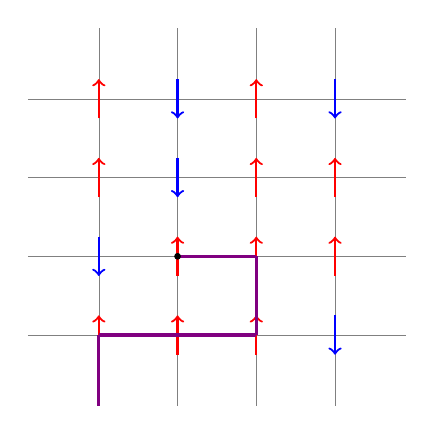
\begin{tikzpicture}
    % grid
    \draw[step=1cm, gray, very thin] (0.1, 0.1) grid (4.9, 4.9);
    % row 1
    \draw[red, ->, thick] (1, 0.75) -- (1, 1.25);
    \draw[red, ->, thick] (2, 0.75) -- (2, 1.25);
    \draw[red, ->, thick] (3, 0.75) -- (3, 1.25);
    \draw[blue, ->, thick] (4, 1.25) -- (4, 0.75);
    % row 2    
    \draw[blue, ->, thick] (1, 2.25) -- (1, 1.75);
    \draw[red, ->, thick] (2, 1.75) -- (2, 2.25);
    \draw[red, ->, thick] (3, 1.75) -- (3, 2.25);
    \draw[red, ->, thick] (4, 1.75) -- (4, 2.25);
    % row 3
    \draw[red, ->, thick] (1, 2.75) -- (1, 3.25);
    \draw[blue, ->, thick] (2, 3.25) -- (2, 2.75);
    \draw[red, ->, thick] (3, 2.75) -- (3, 3.25);
    \draw[red, ->, thick] (4, 2.75) -- (4, 3.25);
    % row 4
    \draw[red, ->, thick] (1, 3.75) -- (1, 4.25);
    \draw[blue, ->, thick] (2, 4.25) -- (2, 3.75);
    \draw[red, ->, thick] (3, 3.75) -- (3, 4.25);
    \draw[blue, ->, thick] (4, 4.25) -- (4, 3.75);
    % worm
    \draw[violet, very thick] (1, 0.1) -- (1, 1);
    \draw[violet, very thick] (1, 1) -- (2, 1);
    \draw[violet, very thick] (2, 1) -- (3, 1);
    \draw[violet, very thick] (3, 1) -- (3, 2);
    \draw[violet, very thick] (3, 2) -- (2, 2);
    \filldraw (2, 2) circle (1pt);
\end{tikzpicture}	

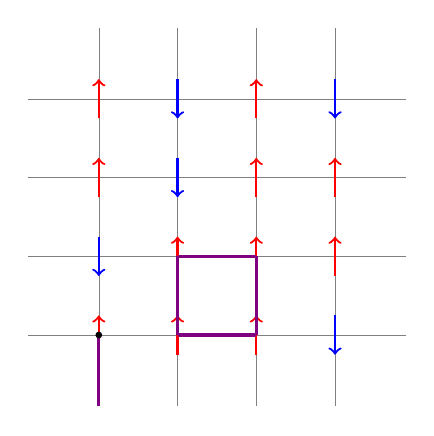
\begin{tikzpicture}
    % grid
    \draw[step=1cm, gray, very thin] (0.1, 0.1) grid (4.9, 4.9);
    % row 1
    \draw[red, ->, thick] (1, 0.75) -- (1, 1.25);
    \draw[red, ->, thick] (2, 0.75) -- (2, 1.25);
    \draw[red, ->, thick] (3, 0.75) -- (3, 1.25);
    \draw[blue, ->, thick] (4, 1.25) -- (4, 0.75);
    % row 2    
    \draw[blue, ->, thick] (1, 2.25) -- (1, 1.75);
    \draw[red, ->, thick] (2, 1.75) -- (2, 2.25);
    \draw[red, ->, thick] (3, 1.75) -- (3, 2.25);
    \draw[red, ->, thick] (4, 1.75) -- (4, 2.25);
    % row 3
    \draw[red, ->, thick] (1, 2.75) -- (1, 3.25);
    \draw[blue, ->, thick] (2, 3.25) -- (2, 2.75);
    \draw[red, ->, thick] (3, 2.75) -- (3, 3.25);
    \draw[red, ->, thick] (4, 2.75) -- (4, 3.25);
    % row 4
    \draw[red, ->, thick] (1, 3.75) -- (1, 4.25);
    \draw[blue, ->, thick] (2, 4.25) -- (2, 3.75);
    \draw[red, ->, thick] (3, 3.75) -- (3, 4.25);
    \draw[blue, ->, thick] (4, 4.25) -- (4, 3.75);
    % worm
    \draw[violet, very thick] (1, 0.1) -- (1, 1);
    \draw[violet, very thick] (2, 1) -- (3, 1);
    \draw[violet, very thick] (3, 1) -- (3, 2);
    \draw[violet, very thick] (3, 2) -- (2, 2);
    \draw[violet, very thick] (2, 2) -- (2, 1);
    \filldraw (1, 1) circle (1pt);
\end{tikzpicture}

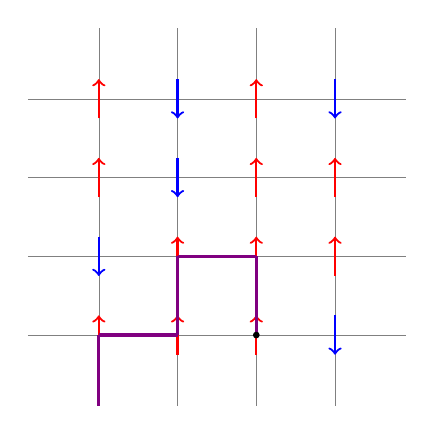
\begin{tikzpicture}
    % grid
    \draw[step=1cm, gray, very thin] (0.1, 0.1) grid (4.9, 4.9);
    % row 1
    \draw[red, ->, thick] (1, 0.75) -- (1, 1.25);
    \draw[red, ->, thick] (2, 0.75) -- (2, 1.25);
    \draw[red, ->, thick] (3, 0.75) -- (3, 1.25);
    \draw[blue, ->, thick] (4, 1.25) -- (4, 0.75);
    % row 2    
    \draw[blue, ->, thick] (1, 2.25) -- (1, 1.75);
    \draw[red, ->, thick] (2, 1.75) -- (2, 2.25);
    \draw[red, ->, thick] (3, 1.75) -- (3, 2.25);
    \draw[red, ->, thick] (4, 1.75) -- (4, 2.25);
    % row 3
    \draw[red, ->, thick] (1, 2.75) -- (1, 3.25);
    \draw[blue, ->, thick] (2, 3.25) -- (2, 2.75);
    \draw[red, ->, thick] (3, 2.75) -- (3, 3.25);
    \draw[red, ->, thick] (4, 2.75) -- (4, 3.25);
    % row 4
    \draw[red, ->, thick] (1, 3.75) -- (1, 4.25);
    \draw[blue, ->, thick] (2, 4.25) -- (2, 3.75);
    \draw[red, ->, thick] (3, 3.75) -- (3, 4.25);
    \draw[blue, ->, thick] (4, 4.25) -- (4, 3.75);
    % worm
    \draw[violet, very thick] (1, 0.1) -- (1, 1);
    \draw[violet, very thick] (1, 1) -- (2, 1);
    \draw[violet, very thick] (3, 1) -- (3, 2);
    \draw[violet, very thick] (3, 2) -- (2, 2);
    \draw[violet, very thick] (2, 2) -- (2, 1);
    \filldraw (3, 1) circle (1pt);
\end{tikzpicture}

\end{document}  
